\section{Best ever achieved emittance}

The quest to minimize the drive beam emittance continued all along the CTF3 lifetime 
and indeed for the nominal factor 8 recombined beam the lowest value was recorded on the very last day of operation.
The measurements presented here are the best values achieved at given location. 
The values correspond to 1~\textsigma~ normalized emittance.

The machine drifts made this tusk very difficult. 
During the initial years it was virtually impossible to systematically optimize the beam optics 
and the orbit because measurements and optimizations were becoming obsolete within less than one hour.
Only in 2014 the machine achieved sufficient stability levels so the beam performance 
optimizations gave the expected results and the improved beam quality could be maintained 
over time. 

Required optimizations at the injector level, 
but also relatively frequent failures of the RF sources,
meant that beam parameters in the injector and the linac were periodically changed.
These made the previous optimizations invalid and 
meant that the setup had to be redone all along the machine.
Here important factor was also the time needed for measurements and preparation of the corrections.
The most crucial measurements, quadrupolar scans and dispersion, took tens of minutes.
Naturally, the software tools helped to automatize most of the tasks, 
however, they were developed already during the machine operation
and some of them become available relatively late.


\subsection{Emittance evolution \label{sec:emittancemeasured}}

Table~\ref{tab:emittancesummary} lists the achieved emittances along the machine.
One can find more dowstream values are sometimes smaller than the upstream ones.
This observetion was not uncommon at CTF3 and there are several effects that explain this.
First, the measured beam size is affected by nonlinearites and 
they can be differently pronounced at different locations. It was specially true 
for the drive beam with 0.6\% energy spread combined with a strong isochronous optics.
Socond, it can not excluded that some small part of the beam was scraped in the transport.
Even though the calibration of the BPMs was carefully done, 
their overal accuracy was at the order of 10\%. 
Finally, the systematic errors of the quadrupolar scans is within tens of percent. 
\todo[inline]{Add this to QS section (paragraph about QuadScan systematic uncertainty) }
Repeating the same measurement normally was giving results with \textpm5\% spread and 
using different ranges for quadrupole strengths sometimes gave 50\% different results.
Of course, this was an indication of an error in the hardware or in the computer program.
It was verified multiple times and the software was tested with simulated data.

% 1.5GHz 
  % Linac 
    %  H  59 with switches http://elogbook.cern.ch/eLogbook/eLogbook.jsp?lgbk=100&date=20160509
    %  V  40     several measurements on that day (following day 70/45 H/V)
    %  H  57  http://elogbook.cern.ch/eLogbook/event_viewer.jsp?eventId=1794890 (2014)
    %  V  51  http://elogbook.cern.ch/eLogbook/event_viewer.jsp?eventId=2118848  30-May-2016
  % DLin 
    %  H  57  http://elogbook.cern.ch/eLogbook/event_viewer.jsp?eventId=2225942
    %  H  68  http://elogbook.cern.ch/eLogbook/event_viewer.jsp?eventId=2113239 and 67 the same day (18-May-2016)
    %  H  67  http://elogbook.cern.ch/eLogbook/event_viewer.jsp?eventId=1797783 (03-Apr-2014)
    %  H  72  http://elogbook.cern.ch/eLogbook/event_viewer.jsp?eventId=1798385 (14-Apr-2014)
    %  V  76  http://elogbook.cern.ch/eLogbook/event_viewer.jsp?eventId=2113196 and 2 other measurements at 90 (18-May-2016)
    %  V  63  http://elogbook.cern.ch/eLogbook/event_viewer.jsp?eventId=1798386 (14-Apr-2014)
    %  H  55  http://elogbook.cern.ch/eLogbook/event_viewer.jsp?eventId=1854639  (18-Nov-2014)
    %  V  gingin 40-50 series of crappy scans  17-05-2016
  % DLex 
    %  H  91  http://elogbook.cern.ch/eLogbook/event_viewer.jsp?eventId=2225940  (06-Dec-2016)
    %  V 125  http://elogbook.cern.ch/eLogbook/event_viewer.jsp?eventId=2225941  (06-Dec-2016)
    %  V  76  http://elogbook.cern.ch/eLogbook/event_viewer.jsp?eventId=1797777  (2014)
    % 
  %
  % CRej 
    % H 65   http://elogbook.cern.ch/eLogbook/event_viewer.jsp?eventId=2218270 22-Nov-2016
    % V 90   http://elogbook.cern.ch/eLogbook/event_viewer.jsp?eventId=2228055
  % CLEX
    %  H 270  http://elogbook.cern.ch/eLogbook/event_viewer.jsp?eventId=1796347
    %  V 110  http://elogbook.cern.ch/eLogbook/event_viewer.jsp?eventId=1796338 (2014)
    %  H 150  http://elogbook.cern.ch/eLogbook/event_viewer.jsp?eventId=1796888 
    %  V 100   --//--
    

% 3GHz
  % Linac
    %         no good measurements in 2016 
    %  H  58  http://elogbook.cern.ch/eLogbook/event_viewer.jsp?eventId=1833447   (2014)
    %  H  53  http://elogbook.cern.ch/eLogbook/event_viewer.jsp?eventId=1958366  (2015.07.01)
    %         two other ones at 60
    %  V  56  http://elogbook.cern.ch/eLogbook/event_viewer.jsp?eventId=1833452 
    %  V  41-50  http://elogbook.cern.ch/eLogbook/event_viewer.jsp?eventId=1958361 and around (2015.07.01)
    %            1 measurment at 41 and several others at 50-51
  % DLin 
    % H  66,75 http://elogbook.cern.ch/eLogbook/eLogbook.jsp?lgbk=100&date=20160726 (2016)  Other sets confirming these results on 0726 
    % V  75,80   on 0727 http://elogbook.cern.ch/eLogbook/eLogbook.jsp?lgbk=100&date=20160727 (2016)
  %               on 0807 http://elogbook.cern.ch/eLogbook/event_viewer.jsp?eventId=2156401 (2016)
  % CRej 3GHz 
    % H 105 http://elogbook.cern.ch/eLogbook/event_viewer.jsp?eventId=2227257 09-Dec-2016
    % H 79  http://elogbook.cern.ch/eLogbook/event_viewer.jsp?eventId=2227299 09-Dec-2016
    % H 80  http://elogbook.cern.ch/eLogbook/event_viewer.jsp?eventId=2227415 09-Dec-2016
    % V 47  http://elogbook.cern.ch/eLogbook/event_viewer.jsp?eventId=2227258 09-Dec-2016
    % V 64  http://elogbook.cern.ch/eLogbook/event_viewer.jsp?eventId=2181929 20-Sep-2016
  %  
  % CLEX 
    % H 112 (2016) http://elogbook.cern.ch/eLogbook/event_viewer.jsp?eventId=2177822
    % H 83  (2015) http://elogbook.cern.ch/eLogbook/event_viewer.jsp?eventId=1959321
    % V 68  (2015) http://elogbook.cern.ch/eLogbook/event_viewer.jsp?eventId=1959324
    % V     (2016) http://elogbook.cern.ch/eLogbook/eLogbook.jsp?lgbk=100&date=20160920  
    %               series of 3 qs but need to be merged and reprocessed 
    % V 73   http://elogbook.cern.ch/eLogbook/event_viewer.jsp?eventId=2161778  (2016) 
    %       not the best one, can be combined with previous ones 
\todo[inline]{There is problem with 1.5GHz measurements in CC, in 2016 there is not much, and before camera was badly calibrated.}
\begin{table}[h]
 \centering
  \begin{tabular}{lcccc}
    \hline
    {\multirow{3}{*}{Location}}& \multicolumn{4}{c}{Emittance [mm mrad]}  \\
                               & \multicolumn{2}{c}{1.5~GHz}  & \multicolumn{2}{c}{3~GHz}           \\
                               & Horizontal   &   Vertical  & Horizontal & Vertical       \\
    \hline \hline
               Linac           &  59   &  40  &  53  &  41     \\
               DL injection    &  57   &  76  &  66  &  75     \\
               DL extraction   &  90   & 126  &   -  &   -     \\
               CR extraction   &  65   &  90  &  79  &  47     \\
               CLEX            & 150   & 100  &  83  &  68     \\
    \hline
  \end{tabular}
\caption{Record emittance measurements of a not combined drive beam along CTF3.}
\label{tab:emittancesummary}
\end{table}
% f4 intensity comparison between Straight and DL http://elogbook.cern.ch/eLogbook/attach_viewer.jsp?attach_id=1602813

Table \ref{tab:emittancevsturns} shows the emittance growth in function of turns
that the beam made in the Combiner Ring. We quote growth in percents because 
the screen was not accurately calibrated during this particular measurement. 

Behind the Combiner Ring, for the beam making only half a turn, emittance was 80~mm~mrad.
For the beam making 3 or 4 turns it was 120~mm~mrad in the best case, 
and routinly it was in range of 140-170~mm~mrad. 
The principal reason was dispersion wave created by the RF bump on the fourth turn.
In the vertical plane the growth was much smaller and values below 80~mm~mrad were measured.
In CLEX the lowest values ranged between 80 and 140 in function of turns in the ring. 
In the horizontal plane the emittance was growing in function of turns to 150 - 200~mm~mrad
and it was not possible to reduce it simultaneously for all the sub-trains. 
Finally it was understood that the beam was loosing energy in the combiner ring
due to the orbit that was not properly centered in the RF~deflectors. 
It was found only during the last months of the operation and 
when it was corrected the combined beam emittance was reduced (factor 4 from 350 to 250~mm~mrad), 
however, there was not enough time to repeat the detailed turn-by-turn emittance measurements at CLEX.


%%%%%%%%%%%%%%%%%%%%%%%%%%%%%%%%%%%%%%%%%%%%%%%%%%%%%%%%%%%%%
%%%%%%%%%%%%%%%%%%%%%%%%%%%%%%%%%%%%%%%%%%%%%%%%%%%%%%%%%%%%%
%%%%%%%%%%%%%%%%%%%%%%%%%%%%%%%%%%%%%%%%%%%%%%%%%%%%%%%%%%%%%
%%%%%%%%%%%%%%%%%%%%%%%%%%%%%%%%%%%%%%%%%%%%%%%%%%%%%%%%%%%%%
 %% Transverse closure between different turns in CR
% summary of quadscans on 3/12/2015 for a factor 2 beam circulating in CR (and final factor 8)
% study in girder 271 with no intervention on CR closure.
%%  %turns   betax           alfax          emitx                   chix    file
%%  0.5     2.84 +/- 0.45   -2.78 +/- 0.49  120.43 +/- 7.56         91.61   eh7363020342.dat
%%  1.5     4.59 +/- 0.38   -3.20 +/- 0.28  228.26 +/- 8.04         28.73   eh7363020523.dat   USELESS
%%  2.5     3.83 +/- 0.51   -2.99 +/- 0.43  175.98 +/- 9.69         198.55  eh7363020539.dat
%%  3.5     6.93 +/- 2.06   -5.13 +/- 1.59  256.27 +/- 35.13        366.33  eh7363020297.dat
%%  fact8   5.71 +/- 0.39   -4.48 +/- 0.32  399.44 +/- 13.28        47.44   eh7363020367.dat
%%  %Vertical scan
%%  %turns   betay   alfay   emity   chiy    file
%%  0.5     3.30 +/- 0.29   -0.86 +/- 0.10  23.15 +/- 0.85  26.15   ev7363020472.dat
%%  1.5     4.85 +/- 0.62   -1.09 +/- 0.16  23.40 +/- 1.18  193.92  ev7363020510.dat
%%  2.5     2.82 +/- 0.30   -0.41 +/- 0.09  35.36 +/- 1.76  30.99   ev7363020572.dat
%%  3.5     not done :(
%%  fact8   3.19 +/- 0.38   -0.87 +/- 0.14  65.33 +/- 3.10  32.43   ev7363020382.dat
%%  
%%  %%  
%%  %% Tobias did some study on 271 on 23/10/2015 (3GHz beam)
%%  % vertical
%%  filename  =  'ev7362604057.dat'; % 1 turn in ring ey = 24
%%  filename  =  'ev7362604252.dat'; % 2 turn in ring ey = 38
%%  filename  =  'ev7362604215.dat'; % 3 turn in ring ey = 57
%%  filename  =  'ev7362604169.dat'; % 4 turn in ring ey = 38
%%  filename  =  'ev7362604310.dat'; % 4 turn in ring ey = 42
%%  % horizontal
%%  filename  =  'eh7362604389.dat'; % 1 turn in ring ex = 72
%%  filename  =  'eh7362604407.dat'; % 2 turn in ring ex = 99
%%  filename  =  'eh7362604441.dat'; % 3 turn in ring ex = 98
%%  filename  =  'eh7362604352.dat   % 4 turn in ring ex = 157
%%  filename = 'eh7362604507.dat'; % 4 turn in ring ex=281
%%  % combined beam
%%  filename = 'eh7362606256.dat'; % H 234
%%  filename = 'ev7362606282.dat'; % V 67
%%  
%%  
%%  %% effect of DL beam on factor 8 in girder 300.
%%  % girder 300 factor 8 (15/12/2015 morning) HV with/without DL beam.
%%  filename = 'eh7363134691.dat'; -%%  466 emit
%%  filename = 'ev7363134720.dat'; -%%  199 emit
%%  % same, but killing DL
%%  filename = 'eh7363134732.dat'; -%%  371 emit
%%  filename = 'ev7363134743.dat'; -%%  194 emit
%%         
%%  09.12.2016
%%  H  1T 106  http://elogbook.cern.ch/eLogbook/event_viewer.jsp?eventId=2227257  beta x   11.78 +/- 1.04 alpha x  -8.25 +/- 0.73 emittance x 105.97 +/- 3.81 
%%  H  2T 108  http://elogbook.cern.ch/eLogbook/event_viewer.jsp?eventId=2227254  beta x    8.35 +/- 1.60 alpha x  -5.98 +/- 1.18 emittance x 108.18 +/- 8.31 
%%  H  3T 176  http://elogbook.cern.ch/eLogbook/event_viewer.jsp?eventId=2227250  beta x    6.42 +/- 1.50 alpha x  -4.38 +/- 1.08 emittance x 176.06 +/- 15.55 
%%  H  4T 158  http://elogbook.cern.ch/eLogbook/event_viewer.jsp?eventId=2227248  beta x    9.04 +/- 1.20 alpha x  -6.16 +/- 0.84 emittance x 157.88 +/- 8.02
%%           
%%  V  1T  46  http://elogbook.cern.ch/eLogbook/event_viewer.jsp?eventId=2227258  beta y    9.55 +/- 0.55 alpha y  -2.44 +/- 0.16 emittance y 45.56 +/- 1.60 
%%  V  2T  97  http://elogbook.cern.ch/eLogbook/event_viewer.jsp?eventId=2227255  beta y    5.07 +/- 0.21 alpha y  -1.53 +/- 0.07 emittance y 96.82 +/- 1.64 
%%  V  3T  99  http://elogbook.cern.ch/eLogbook/event_viewer.jsp?eventId=2227252  beta y   11.02 +/- 1.43 alpha y  -3.89 +/- 0.52 emittance y 98.72 +/- 5.91
%%  V  4T  54  http://elogbook.cern.ch/eLogbook/event_viewer.jsp?eventId=2227249  beta y    5.25 +/- 0.28 alpha y  -1.66 +/- 0.09 emittance y 54.37 +/- 1.15 





% 2016 Dec 12 turns
\begin{table}[]
 \centering
  \begin{tabular}{ccc}
    \hline
     Turn  & Horizontal & Vertical \\
           & [\%]       & [\%] \\
    \hline
    \hline                      
     1\nicefrac{1}{2}  &  2   & 53	 \\
     2\nicefrac{1}{2}  &  40  & 54	 \\
     3\nicefrac{1}{2}  &  33  & 16	 \\

    \hline
  \end{tabular}
\caption{Emittance growth of not combined drive beam in function of number of turns in CR with respect 
         of the beam extracted after \nicefrac{1}{2} turn.}
\label{tab:emittancevsturns}
\end{table}
%% Using data of 23/10/2015
%\begin{table}[]
% \centering
%  \begin{tabular}{ccc}
%    \hline
%    Turn  & Horizontal & Vertical \\
%           & [\%]       & [\%] \\
%    \hline
%    \hline
%     1\nicefrac{1}{2}  &  38   &   58    \\
%     2\nicefrac{1}{2}  &  36   &   138   \\
%     3\nicefrac{1}{2}  &  118  &   58    \\
%    \hline
%  \end{tabular}
%\caption{Emittance growth of not combined drive beam in function of number of turns in CR with respect 
%         of the beam extracted after \nicefrac{1}{2} turn.}
%label{tab:emittancevsturns}
%\end{table}



\subsubsection{Transverse matching}

Example results of the transverse matching for the beam combined in the Delay Loop is 
shown in Table~\ref{tab:DLTransvClosure}. 
In the Combiner Ring it was much more difficult to correct the beating,
see section refToSection for the procedure details.
The procedure was very long because all 4 turns had to be measured at each iteration,
such that only one iteration was done in most of the cases. 
Table~\ref{tab:CRTransvClosure} shows example results.

In the Delay Loop it was possible to match the orbits for the combined beams within XX~mm in the horizontal plane 
and XX~mm in the vertical one what corresponds to more or less 0.5~\textsigma~. 
In case of CR it was respectively cXX and cYY? 


%\textbeta-functions Taking into account the stabiliuty of the measured parameters the 

%
% Factor 2  2016-Dec-2016
  % H 152(+154)   http://elogbook.cern.ch/eLogbook/event_viewer.jsp?eventId=2229045
  % V 198         http://elogbook.cern.ch/eLogbook/event_viewer.jsp?eventId=2229046
% DL 08-Dec-2015
  % H st 102  7.61  -0.78   http://elogbook.cern.ch/eLogbook/event_viewer.jsp?eventId=2053610
  % H dl 112  8.92  -0.60   http://elogbook.cern.ch/eLogbook/event_viewer.jsp?eventId=2053605
  % V st  55  2.36   0.01   http://elogbook.cern.ch/eLogbook/event_viewer.jsp?eventId=2053609
  % V dl  66  4.59  -0.03   http://elogbook.cern.ch/eLogbook/event_viewer.jsp?eventId=2053611
  
%  DL 2016-Nov-21
  % H x2 beta x   7.92 +/- 0.31  alpha x  -0.58 +/- 0.03  emittance x 128.05 +/- 2.15
  % H st beta x   7.67 +/- 0.27  alpha x  -0.32 +/- 0.02  emittance x 63.36 +/- 0.88
  % H dl beta x   10.40 +/- 1.75 alpha x  -0.70 +/- 0.14  emittance x 225.43 +/- 17.95 

%  DL 06-Dec-2016
  % H st beta x   6.32 +/- 0.25 alpha x  -0.24 +/- 0.02  emittance x 55.63 +/- 0.83      http://elogbook.cern.ch/eLogbook/event_viewer.jsp?eventId=2225942
  % H dl beta x   6.31 +/- 0.90 alpha x  -0.80 +/- 0.11  emittance x 90.64 +/- 4.87      http://elogbook.cern.ch/eLogbook/event_viewer.jsp?eventId=2225941
  % H x2 beta x   7.00 +/- 0.83 alpha x  -0.25 +/- 0.07  emittance x 120.07 +/- 5.64     http://elogbook.cern.ch/eLogbook/event_viewer.jsp?eventId=2225951
  % 
  % V st beta y   9.01 +/- 0.11 alpha y  -0.15 +/- 0.01  emittance y 188.75 +/- 1.27     http://elogbook.cern.ch/eLogbook/event_viewer.jsp?eventId=2225943
  % V dl beta y   9.18 +/- 0.70 alpha y  -0.65 +/- 0.06  emittance y 125.68 +/- 5.70     http://elogbook.cern.ch/eLogbook/event_viewer.jsp?eventId=2225942
  % V x2 beta y   9.33 +/- 0.52 alpha y  -0.33 +/- 0.04  emittance y 182.51 +/- 5.81     http://elogbook.cern.ch/eLogbook/event_viewer.jsp?eventId=2225952
\begin{table}[h!]
 \centering
 \caption{Achieved Twiss Parameters closure for the Delay Loop}
 \begin{tabular}{ l c c c c c}
  \hline
    	& $\beta_x$ [m]   & $\alpha_y$   & $\beta_y$ [m]  & $\alpha_y$         \\
  Bypass beam	& 6.32 \textpm ~0.25  & -0.24 \textpm 0.02 & 9.01 \textpm 0.11 & -0.15 \textpm 0.01  \\
  Delayed beam	& 6.31 \textpm ~0.90  & -0.80 \textpm 0.11 & 9.18 \textpm 0.70 & -0.65 \textpm 0.06  \\
  Combined beam	& 7.00 \textpm ~0.83  & -0.25 \textpm 0.07 & 9.33 \textpm 0.52 & -0.33 \textpm 0.04  \\
  \hline
 \end{tabular}
 \label{tab:DLTransvClosure}
\end{table}


\begin{table}[h!]
 \centering
 \caption{Example results for Twiss Parameters closure for the Combiner Ring}
 \begin{tabular}{ l c c c c c}
  \hline
    Turn	& $\beta_x$ [m]   & $\alpha_y$   & $\beta_y$ [m]  & $\alpha_y$         \\
  \nicefrac{1}{2}	& 11.78 \textpm ~1.04  & -8.25 \textpm ~0.73 &  9.55 \textpm ~0.55 & -2.44 \textpm ~0.16  \\
  1\nicefrac{1}{2}  &  8.35 \textpm ~1.60  & -5.98 \textpm ~1.18 &  5.07 \textpm ~0.21 & -1.53 \textpm ~0.07  \\
  2\nicefrac{1}{2}  &  6.42 \textpm ~1.50  & -4.38 \textpm ~1.08 & 11.02 \textpm ~1.43 & -3.89 \textpm ~0.52  \\
  3\nicefrac{1}{2}  &  9.04 \textpm ~1.20  & -6.16 \textpm ~0.84 &  5.25 \textpm ~0.28 & -1.66 \textpm ~0.09  \\
  \hline
 \end{tabular}
 \label{tab:CRTransvClosure}
\end{table}





\subsection{Combined beam emittance}

%%%%%%%%%%%%%%%%%%%%%%%%%%%%%%%%%%%%%%%%%%%%%%%%%%%%%%%%%%%%%%%%%%%%%%%%%%%%%%%%%%%%%%%%%%%%%%%%%%%%%
% F8 girder 27
%%%%%%%%%%%%%%%%%%%%%%%%%%%%%%%%%%%%%%%%%%%%%%%%%%%%%%%%%%%%%%%%%%%%%%%%%%%%%%%%%%%%%%%%%%%%%%%%%%%%%
% Vertical 120 mm mrad with ~27A beam 
%    http://elogbook.cern.ch/eLogbook/event_viewer.jsp?eventId=2228935
%     corresponding transmission meas http://elogbook.cern.ch/eLogbook/event_viewer.jsp?eventId=2228936
% V 138 mm mrad                    on 2014 May 13 12h09  http://elogbook.cern.ch/eLogbook/event_viewer.jsp?eventId=1800616


The lowest achieved emittance for factor 8 recombined beam  was 243~mm~mrad for horizontal plane
and 120~mm~mrad for vertical plane.
Figure~\ref{fig:record_low_factor8_girder27} shows the results of the respective quadrupole scan measurements 
at the beginning of the TL2 line with screen CC.MTV0253
(see Fig.~\ref{fig:layout_screens} depicting location of the screens).
It needs to be mentioned that with the setting yielding the record horizontal emittance 
the beam was not transported losslessly and measured beam current was around 24-25~A.
The vertical emittance was confirmed with the nominal 28~A beam.
By changing the pulse length from the gun it was verified that all the subtrains were contributing 
to the measured profiles and the integrated light intensity linearly increased with the pulse length.
Unfortunately, because drifts of various beam parameters, maintaining such emittance was not possible 
for longer periods and in average emittances were around 400/180~mm~mrad (horizontal/vertical).


\begin{figure}[!h]
 \begin{center}
  \subfloat[]  %On the plot 16 Dec 2016 14:18
   {\includegraphics[width=0.41\columnwidth]{Emi_F8_H_CC_record.eps}} %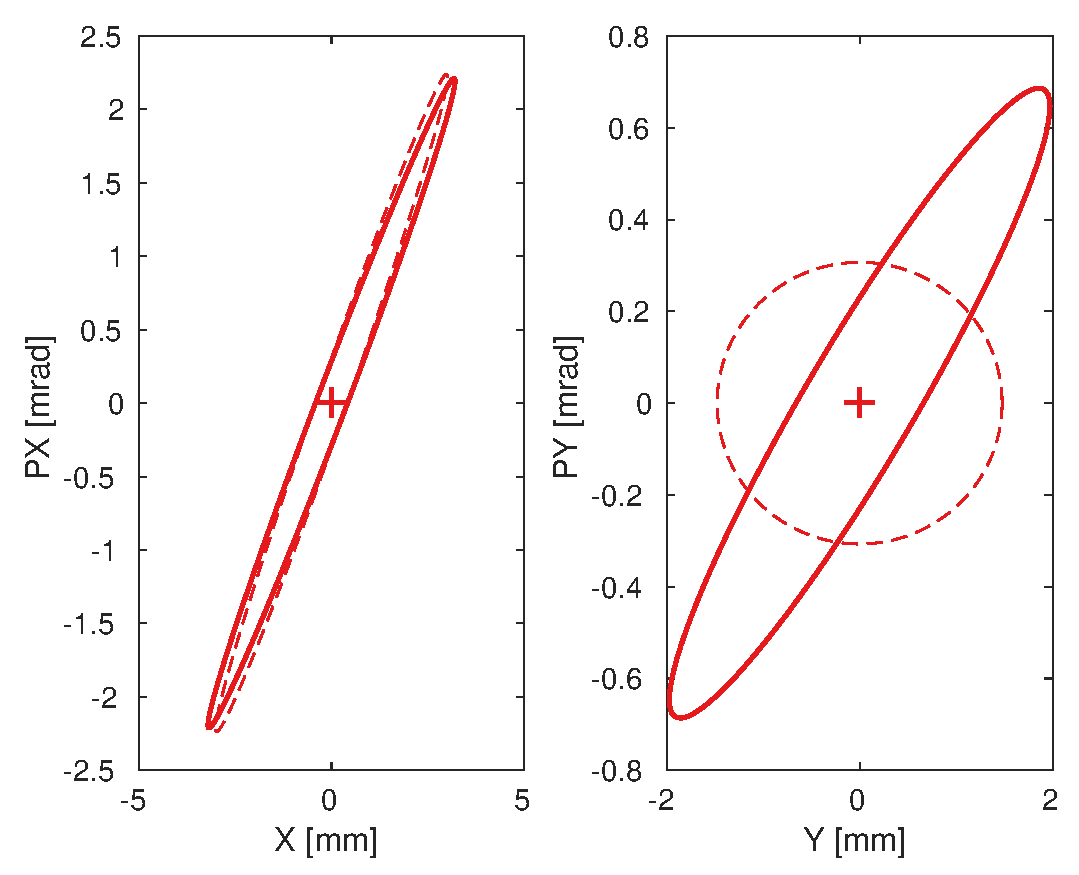
\includegraphics[height=8.4cm]{figs/quadscans/factor8_271.eps}
 \subfloat[]   %On the plot 15 Dec 2016 18:56
   {\includegraphics[width=0.405\columnwidth]{Emi_F8_V_CC_record.eps}}
 \end{center}
 \caption{Results of the quadrupolar scans for factor 8 recombined beam in (a) horizontal and (b) vertical plane.}
 \label{fig:record_low_factor8_girder27}
\end{figure}



Figure~\ref{fig:record_low_factor8_30} presents the measuremnts obtained with screen CC.MTV0930 
located at CLEX just in front of TBL and TBTS line. 
In the vertical plane it relatively easy to achieve emittance below 150~mm~mrad, and the record was 119~mm~mrad.
On the other hand, the beam transport through the achromatic chicanes in the TL2 (the vertical and the horizontal one)
provoked additional emittance growth in the horizontal plane. 
For the setting that yielded the lowest emittance at CC.MTV0253, which was on the last day of CTF3 operation,
technical problems make measurement at CLEX impossible. 
On previous days it was measured 520~mm~mrad while at CC.MTV0253 it was approximately 300~mm~mrad 
(three consequtive measurements ranged between 283 and 329~mm~mrad).
At this location the lowest ever measured value of 430~mm~mrad was recorded in April 2014, however, 
it was not confirmed by the consecutive measurements (three other measurements were above 600~mm~mrad).


% The best I find
% H 467 mm mrad  eh7363134691.dat  on 2015 Dec 15 11h16  http://elogbook.cern.ch/eLogbook/event_viewer.jsp?eventId=2056049
%                     on the day above V was 200: ev7363134720.dat http://elogbook.cern.ch/eLogbook/event_viewer.jsp?eventId=2056051               
% H 515 mm mrad  eh7366777416.dat  on 2016 dec 13 17h50  http://elogbook.cern.ch/eLogbook/event_viewer.jsp?eventId=2228399
% Good vertical 
% V 142 mm mrad  ev7366777452.dat  on 2016 Dec 13 17h54  http://elogbook.cern.ch/eLogbook/event_viewer.jsp?eventId=2228401
%        Horizontal was not done on the last day (the machine started drifting away in a crazy way - let's say technical problems)
% V 144 mm mrad  ev7357147045.dat   on 2014 Apr 25 16h56   http://elogbook.cern.ch/eLogbook/event_viewer.jsp?eventId=1799099
%                     on the day above H was 750 mm mrad
% V 148 mm mrad                     on 2014 Apr 29 18h09  http://elogbook.cern.ch/eLogbook/event_viewer.jsp?eventId=1799325


%On the plot 
% H 431 mm mrad  eh7357187482_cleaned.dat  on 2014 Apr 29 17h56  http://elogbook.cern.ch/eLogbook/event_viewer.jsp?eventId=1799323
% V 119 mm mrad  ev7357186955_cleaned.dat  on 2014 Apr 29 16h39  http://elogbook.cern.ch/eLogbook/event_viewer.jsp?eventId=1799295
\begin{figure}[!h]
\begin{center}

  \subfloat[]  
   { 
    %\includegraphics[height=8.4cm,natwidth=1600,natheight=1200]{eh7363134691.png}
    \includegraphics[width=0.41\columnwidth]{Emi_F8_H_CLEX_record_420.eps}
   }
  \subfloat[]  
   { 
    %\includegraphics[height=8.4cm,natwidth=345,natheight=702]{combined_factor8_girder30_vertical_20140425165614.png}
    \includegraphics[width=0.43\columnwidth]{Emi_F8_V_CLEX_record_122.eps}
   }

\end{center}
\caption{Quadrupolar scans at CC.MTV0970 for factor 8 combined beam.}
\label{fig:record_low_factor8_30}
\end{figure}



%%%%%%%%%%%%%%%%%%%%%%%%%%%%%%%%%%%%%%%%%%%%%%%%%%%%%%%%%%%%%%%%%%%%%%%%%%%%%%%%%%%%%%%%%%%%%%%%%%%%%
%%%%%%%%%%%%%%%%%%%%%%%%%%%%%%%%%%%%%%%%%%%%%%%%%%%%%%%%%%%%%%%%%%%%%%%%%%%%%%%%%%%%%%%%%%%%%%%%%%%%%
%%%%%%%%%%%%%%%%%%%%%%%%%%%%%%%%%%%%%%%%%%%%%%%%%%%%%%%%%%%%%%%%%%%%%%%%%%%%%%%%%%%%%%%%%%%%%%%%%%%%%

%\subsection{Factor 4}
%%%%%%%%%%%%%%%%%%%%%%%%%%%%%%%%%%%%%%%%%%%%%%%%%%%%%%%%%%%%%%%%%%%%%%

Figures~\ref{fig:record_low_factor4_girder27} and~\ref{fig:record_low_factor4_girder30} show 
the record measurements of factor 4 combined beam at the exit of the Combiner Ring and at CLEX, respectively.
At the extraction of the Combiner Ring 148~mm~mrad in horizontal plane was and 91~mm~mrad in the vertical one
were achieved and at CLEX it was 173 and 96 respectively.

%%%%%%%%%%%%%%%%%%%%%%%%%%%%%%%%%%%%%%%%%%%%%%%%%%%%%%%%%%%%%%%%%%%%%%


% On the plot :
% H 145 mm mrad on 2016 Dec 09 10h31 eh7366734365.dat  http://elogbook.cern.ch/eLogbook/event_viewer.jsp?eventId=2227021
% V 91  mm mrad on 2016 Dec 09 10h38 ev7366734420.dat  http://elogbook.cern.ch/eLogbook/event_viewer.jsp?eventId=2227025 

\begin{figure}[!h]
 \begin{center}
  \subfloat[]  %On the plot 16 Dec 2016 14:18
   { 
     \includegraphics[width=0.405\columnwidth]{Emi_F4_H_CC_record.eps}
   }
  \subfloat[]  %On the plot 
   { 
     \includegraphics[width=0.43\columnwidth]{Emi_F4_V_CC_record.eps}
   }
   
 \end{center}
\caption{Factor 4, girder 27}
\label{fig:record_low_factor4_girder27}
\end{figure}


%  Other good data                                   
% H 75 mm mrad on 2012 Oct 18 10h27  http://elogbook.cern.ch/eLogbook/event_viewer.jsp?eventId=1721059  combined_factor4_girder27_20121018103111.png


%%%%%%%%%%%%%%%%%%%%%%%%%%%%%%%%%%%%%%%%%%%%%%%%%%%%%%%%%%%%%%%%%%%%%%%%%%%%%%%%%%%%%%%%%%%%%%%%%%%%%
%%%%%%%%%%%%%%%%%%%%%%%%%%%%%%%%%%%%%%%%%%%%%%%%%%%%%%%%%%%%%%%%%%%%%%%%%%%%
%
%

% On the plot :
%   H 173 mm mrad on 2012 Dec 7  17h00
%   V 96  mm mrad on 2012 Nov 08 11h03

\begin{figure}[!h]
  \begin{center}
    \subfloat[]  %On the plot 
     { 
       %\includegraphics[height=8.4cm,natwidth=404,natheight=714]{combined_factor4_girder30_horizontal.png}
       \includegraphics[height=10.4cm]{combined_factor4_girder30_horizontal.png}
     }
    \subfloat[]  %On the plot 
     { 
       %\includegraphics[height=8.4cm,natwidth=439,natheight=712]{combined_factor4_girder30_vertical_20121108110306.png}
       \includegraphics[height=10.4cm]{combined_factor4_girder30_vertical_20121108110306.png}
     }

  \end{center}
\caption{Factor 4, girder 30}
\label{fig:record_low_factor4_girder30}
\end{figure}


%  Other good data                                   
%  H 278 mm mrad                  on  2012 Nov 08 11h06  http://elogbook.cern.ch/eLogbook/event_viewer.jsp?eventId=1734866
%  H 278 mm mrad eh7366733975.dat on  2016 Dec 09 09h33  http://elogbook.cern.ch/eLogbook/event_viewer.jsp?eventId=2226992
%  V 108 mm mrad ev7366733983.dat on  2016 Dec 09 09h34  http://elogbook.cern.ch/eLogbook/event_viewer.jsp?eventId=2226993
%  V 101 mm mrad ev7366733995.dat on  2016 Dec 09 09h36  http://elogbook.cern.ch/eLogbook/event_viewer.jsp?eventId=2226994 (can be combined with the above)
%  V 96  mm mrad ev7366742338.dat on  2016 Dec 10 05h38  http://elogbook.cern.ch/eLogbook/event_viewer.jsp?eventId=2227404
%  V 124 mm mrad                  on  2012 Dec 07 17h53  http://elogbook.cern.ch/eLogbook/event_viewer.jsp?eventId=1755714
%%%%%%%%%%%%%%%%%%%%%%%%%%%%%%%%%%%%%%%%%%%%%%%%%%%%%%%%%%%%%%%%%


% \subsection{Factor 4  End of TBL}
% good data
% H 230 mm mrad  on  2012 Nov 08  15h17    http://elogbook.cern.ch/eLogbook/event_viewer.jsp?eventId=1734994


 

\subsubsection{finalFactor8}{Latest beam quality}
\textbf{Extract from Davides Thesis, 2015 status, maybe something to copy}

The set-up and tuning of the Drive Beam recombination at CTF3 requires generally a few weeks of operation.
Many corrections are necessary, and most of them are coupled with each other.
It is then difficult to say which correction contributed the most to the final recombination quality.
However an interesting measurement was performed on the last day of CTF3 operation of 2015: a factor-8 beam
was finally set up for RF power production in the later CLEX experimental area.
Quadrupole scan measurements were then performed at the end of the TL2 line using the screen CC.MTV0970.
In order to verify the quality of the recombination, at least partially, the measurements were also performed
after dumping all the bunches going via the DL, and so generating an unnatural factor-4 recombination in the
CR.
The measured Twiss parameters for the horizontal and vertical plane and both set-ups are reported in
Table~\ref{tab:finalFactor8Quality}, while a graphical representation of the data collected is shown in
Figure~\ref{fig:finalFactor8Quality}.
%
\begin{figure}[htbp]
\centering
\subfloat[]{
\includegraphics[width=0.45\textwidth]{quadscanComparisonH.eps}
\label{fig:finalFactor8QualityA}
}
\qquad
\subfloat[]{
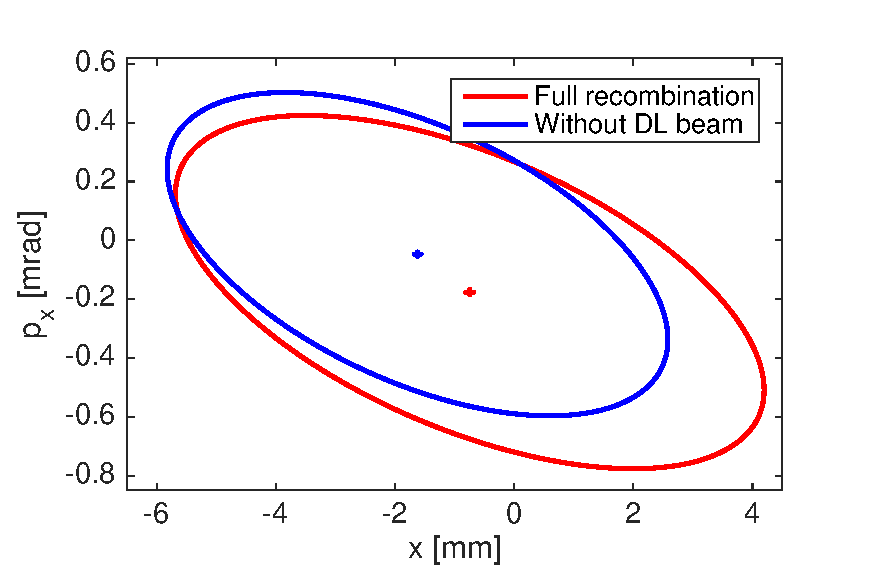
\includegraphics[width=0.45\textwidth]{fwhm_comparisonH.eps}
\label{fig:finalFactor8QualityB}
}
\\
\subfloat[]{
\includegraphics[width=0.45\textwidth]{quadscanComparisonV.eps}
\label{fig:finalFactor8QualityC}
}
\qquad
\subfloat[]{
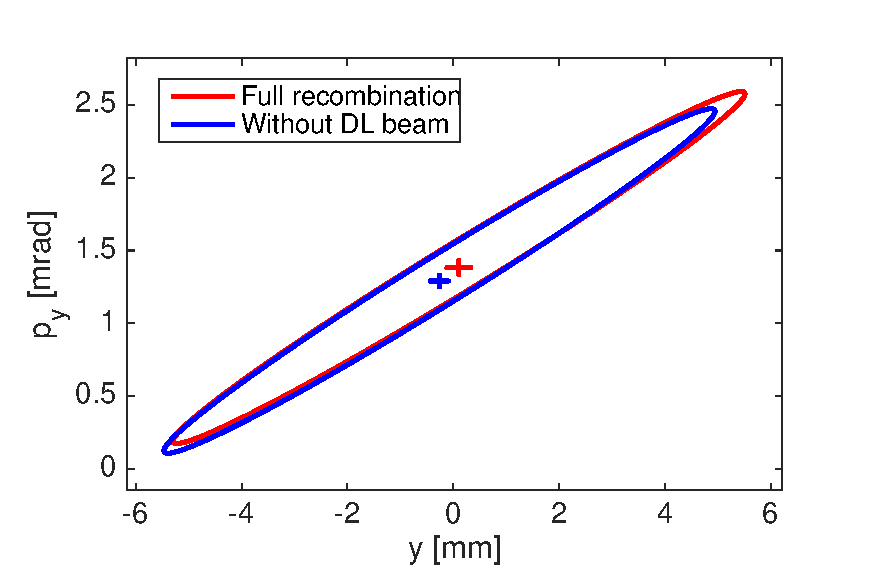
\includegraphics[width=0.45\textwidth]{fwhm_comparisonV.eps}
\label{fig:finalFactor8QualityD}
}
\caption{Beam variance measured at the screen CC.MTV0970 in TL2 as a function of the quadrupole current used
         to perform quadrupole scan measurements
         in the horizontal \protect\subref{fig:finalFactor8QualityA} and vertical
         \protect\subref{fig:finalFactor8QualityC} planes.
         The measured Twiss parameters, reported in Table~\ref{tab:finalFactor8Quality}, are used to
         construct the contour plots in Figures~\protect\subref{fig:finalFactor8QualityB}
         and~\protect\subref{fig:finalFactor8QualityD}.
         These represents  in phase space the FWHM borders of a hypothetical Gaussian beam with covariance
         given by the measured Twiss parameters.
         The red traces are relative to a fully combined factor-8 beam, while in blue are the equivalent
         quadrupole scans but dumping earlier the bunches that normally go via the DL.
}
\label{fig:finalFactor8Quality}
\end{figure}
%
%
\begin{table}[bp]
\centering
\begin{tabular}{l c c c c c c}
\hline
                & $\beta_x$  [m]  &  $\alpha_x$     &  $\epsilon_{Nx}$   [$\mu$m]   & $\beta_y$  [m]  &  $\alpha_y$     &  $\epsilon_{Ny}$   [$\mu$m]    \\
\hline
Factor-8 beam            & $9.9 \pm 1.1$   & $0.7 \pm 0.1$   & $467 \pm 27$       & $27.8 \pm 2.2$   & $-6.1 \pm 0.5$   & $199 \pm 7$ \\
Without DL bunches          & $9.0 \pm 0.5$   & $0.6 \pm 0.1$   & $371 \pm 10$       & $26.4 \pm 2.2$   & $-5.9 \pm 0.5$   & $195 \pm 7$ \\
\hline 
\end{tabular}
\caption{Comparison of the measured Twiss parameter between the final factor-8 beam of 2015 and the same beam
         without the bunches going via the DL.
         The measurements were performed with the screen CC.MTV0970 at the end of DBRC.}
\label{tab:finalFactor8Quality}
\end{table}
%


Note that these measurements were taken after the beam was empirically optimised to obtain the optimum power
production in the CLEX area.
This means that the length of the DL and CR could have been adjusted by acting on the wiggler magnets
installed in the two rings, and also the beam setup could have been manipulated at the injector.
This might have spoiled part of the optimisation performed earlier, but it is interesting to see that in the
vertical plane, normally the plane less affected by energy and ring length variations, there is no
substantial difference with or without the DL bunches.
For the horizontal plane things are not as good, but still an increase of only 25\% in $\epsilon_x$ between
the beam without the DL component and the full factor-8 beam is a sign of good recombination quality.
Moreover from Figure~\ref{fig:finalFactor8Quality}\subref{fig:finalFactor8QualityB} one can see that the
increase in $\epsilon_x$ seems to be due to an orbit error of the order of 2 mm in the DL recombination.
This could be easily explained by the empirical optimisations that were performed to maximise the power
production.







